\documentclass[a4paper,11pt,oneside]{book}
\usepackage[latin1]{inputenc}
\usepackage[english]{babel}
\usepackage{amsfonts}
\usepackage{amsmath}
\usepackage{amssymb,amsmath,color,psfrag}
\usepackage[draft]{graphicx}
\usepackage{cite}
\usepackage{bbm}
\usepackage{float}

\begin{document}
\pagestyle{myheadings}

\thispagestyle{empty}                                                 
\begin{center}                                                            
    \vspace{5mm}                                                           
 {\LARGE UNIVERSIT\`A DEL SALENTO} \\                       
      \vspace{5mm}
\end{center}
\begin{center}
{
\includegraphics[scale=.20]{figs/logo_unisalento}}      
\end{center}
\begin{center}
      \vspace{5mm}
      {\LARGE Facolt\`a di Ingegneria} \\
        \vspace{3mm}
      {\Large Corso di Laurea Magistrale in Computer Engineering} \\
      \vspace{20mm}
      {\LARGE Advanced Control Techniques Project} \\
      \vspace{5mm}{\Large\textbf{DISTRIBUTED GRADIENT ALGORITHM OVER ORDINARY\\ LEAST SQUARES PROBLEM}}                  
      \vspace{15mm}
\end{center}
\begin{flushleft}                                                                              
     {\large Professor: \textbf{\@ Giuseppe Notarstefano}} \\        
      \vspace{13mm}
\end{flushleft}
\begin{flushright}
      {\large Students:}\\
      {\textbf{Salvatore Corvaglia}}\\
 	 {\textbf{Simone Miglietta}}\\
 	 {\textbf{Adriano Luigi Piscopello}}\\
 	 {\textbf{Emanuele Taurino}}\\
\end{flushright}        %capoverso allineato a destra
\begin{center}
\vfill
      {\large Academic year \@2017/2018} \\
\end{center}


\newpage
\thispagestyle{empty}

%%%%%%%%%%%ABSTRACT%%%%%%%%%%%%
\begin{center}
\chapter*{}
\thispagestyle{empty}
{\Huge \textbf{Abstract}}\\
\vspace{15mm}
\end{center}
The project deals with the design and implementation of a distributed
optimization algorithm in order to solve a Supervised Learning (SL) problem.
In particular, the project activity includes to design a software based on Message Passing Interface (MPI) that implements a distributed gradient tracking algorithm. This software will be used to solve a Ordinary Least Squares problem and than the results obtained will be validated through numerical tests over a given dataset. All results will be desplayed graphically to give an immediate idea of the behavior of the agents during the estimate. Finally, the graph of the difference between the solution provided by the sequential algorithm and distributed one will highlight the computing differences between them.

\tableofcontents \thispagestyle{empty}
\listoffigures\thispagestyle{empty}

%%%%%%%%%%INTRODUCTION%%%%%%%%%%
\chapter*{Introduction}
\addcontentsline{toc}{chapter}{Introduction}
\section*{Motivations} 
The objective in studying the distributed optimization problem over a network is to optimize a global function formed by a sum of local functions, using only local computation and communication.
In literature it is unclear how to obtain a faster convergence rate comparable to centralized gradient method's convergence rate when the function is convex and smooth. 

\section*{Contributions}
The software we have developed allows the compute of the minimum of one function $f_i(x): \mathbb{R}^{N} \rightarrow \mathbb{R}$ either using a sequential algorithm or a distributed algorithm. After making the calculations, it allows to graphically visualize both the achievement of the consent and the difference between the result of the sequential algorithm and the distributed one. 
Our software also offers the possibility to split the function into partial sums of functions, one for each agent, or to solve the ordinary least squares problem. Also in this case it is possible to graphically see the difference between the compute made with the sequential algorithm and the distributed one.
The software uses the distributed algorithm that has been proposed by Guannan Qu, Na Li, and it is based on a gradient method descent like algorithm, a kind of algorithm in which each step $x^{k}$, towards the minimum value of the function $f(x)$ (if it has one) is computed as $\min\limits_{x \in R^{N}} f(x)$, where $x^{k+1}= x^{k}- \alpha^{k} D^{k}\nabla f(x^{k})$.
\\In particular the algorithm that Guannan Qu, Na Li takes a function $f_{i}(x)$ for each agent and it calculates next step $x^{k+1}$ using the product of a matrix $D^{k}$ = I  (steepest descend method) with a fixed stepsize $\alpha^{k}= \eta$ (sufficently small) and the estimate of the average gradient $s_{i}^{k}$.


%%%%%%%%%%CAPITOLO%%%%%%%%%%%%%
\chapter{Formulation Of The Problem}
Given a set of agents $\mathcal{N}$ = \{1,2,...,n\} , each of which has
a local convex cost function $f_i(x): \mathbb{R}^{N} \rightarrow \mathbb{R}$ , the objective of
distributed optimization is to find $x$ that minimizes the average of all the functions,
\begin{equation}
\min\limits_{x \in R^{N}} f(x) := \dfrac{1}{n} \sum\limits_{i=1}^{n} f_i (x)
\end{equation}
using local communication and local computation. The local communication is defined through an undirected communication graph $\mathcal{G}$ = (V, E), where the nodes V = $\mathcal{N}$ and the edges E $\subset$ V x V.
Agent $i$ and $j$ can send information to
each other if and only if $i$ and $j$ are connected in graph $\mathcal{G}$.
The local computation means that each agent can only make
his decision based on the local function $f_{i}$ and the information
obtained from his neighbors.
We assume that each $f_{i}$ is convex and $\beta$-smooth.

%%%%%%%%%%CAPITOLO%%%%%%%%%%%%%
\section{Algorithm}
The used algorithm is a consensus based distributed algorithm in which each agent weighs its neighbors' information to compute its local decisions. This process is modeled with a weight matrix W = [$w_{ij}$]$\in \mathbb{R}^{{n}\times{n}}$. In particular, matrix W satisfies:
\begin{enumerate}
\item [a.] For any ($i, j$) $\epsilon$ E, we have $w_{ij} > 0$. For any $i$ $\epsilon$ $\mathcal{N}$, we have $w_{ii} > 0$. For other ($i, j$), we have $w_{ij} = 0$.
\item [b.] Matrix W is doubly stochastic, i.e $\sum\limits_{i^{'}}w_{i^{'}j} = \sum\limits_{j^{'}}w_{ij^{'}} = 1$
\end{enumerate}
In this algorithm, each agent $i$ keeps an estimate of the minimizer $ x_{i}(t)$ $\epsilon $  $\mathbb{R}^{N}$, and another vector $ s_{i}(t)$ $\epsilon $  $\mathbb{R}^{N}$ which is designated to estimate the average gradient, $\dfrac{1}{n} \sum\limits_{i=1}^{n} \nabla f_i (x_{i}(t)) $. Algorithm starts with an arbitrary $x_i(0)$ and with $ s_{i}(0) = \nabla f_i(x_i(0))$, and proceeds according to the following update laws:

\begin{equation}
x_i(t+1) = \sum\limits_{j=1}^{n} w_{ij} x_j(t)-\eta s_i(t)
\end{equation} 

\begin{equation}
s_i(t+1) = \sum\limits_{j=1}^{n} w_{ij} s_j(t) + \nabla f_i(x_i(t+1))-\nabla f_i(x_i(t))
\end{equation}

%%%%%%%%%%CAPITOLO%%%%%%%%%%%%%
\section{Preliminar Steps}
In order to satisfy the requirements in the abstract section, we split the complex problem into more simple tasks. In particular, the steps we made are the followings:
\begin{enumerate}
\item Implementation of the algorithm in Matlab, taking as each node function, the same function $f_i(x): \mathbb{R} \rightarrow \mathbb{R} $, simulating agents with a 'for' cycle. What we expect is that\\ $\min\limits_{x \in \mathbb{R}} f(x) := \dfrac{1}{n} \sum\limits_{i=1}^{n} f_i (x) = \min\limits_{x \in \mathbb{R}} \dfrac{1}{n}*{n}f_i(x) = \min\limits_{x \in \mathbb{R}}f_i(x)$ 
\item Implementation of the algorithm in Matlab similar as before, taking the function $f_i(x): \mathbb{R}^{2} \rightarrow \mathbb{R} $ instead ;
\item Implementation of the algorithm in step [2.] taking the function $f_i(x): \mathbb{R}^{n} \rightarrow \mathbb{R} $ instead;
\item Implementation of the algorithm in Python giving a different function $f_i(x): \mathbb{R}^{2} \rightarrow \mathbb{R} $ to each agent;
\item Implementation of the previous step in Mpi4Py (MPI for Python);
\item Implementation of the algorithm in Python giving a different function $f_i(x): \mathbb{R}^{n} \rightarrow \mathbb{R} $ using Mpi4Py;
\item Feeding software at the point [4.], [5.] and [6.] with the given dataset's points, with the objective of solving the Ordinary Least Squares Problem.     
\end{enumerate}

\newpage
\section{Ordinary Least Squares Problem}
Given a dataset of points $(x_1,y_1),....,(x_n,y_n)$, solving an Ordinary Least Squares Problem means finding the straight line $y = Ax + B$ for which is minimum the quantity:
\begin{equation}
S= \sum\limits_{i=1}^{n}(Ax_i + B - y_i)^2
\end{equation}
For our distributed case, the above equation can be written as : 
\begin{equation}
S= \sum\limits_{i=1}^{n}(X_1x_i + X_2 - y_i)^2
\end{equation}
where $X_1, X_2$ are the consensus values found by our software, and $f_i(x)$ are obtained by splitting (1.5) into partial sums.


\chapter{Implementation}
\section{Pseudocode}
As written before, the first step we took in order to solve the primary problem was to use the algorithm described by Guannan Qu, Na Li  to find the (local) minimum of a generic function $f(x): \mathbb{R} \rightarrow \mathbb{R} $. In particular if $f(x)$ is convex, then every local minimum is a global minimum.
We implemented this algorithm in Matlab as following:
\small
{\linespread{0.66}\selectfont
\begin{itemize}
\item[] define $f_{i}(x)$;
\item[] define number of agents $N$;
\item[] generate $Adj$ matrix;
\item[] loop until $Adj$ is strongly connected;
\item[] generate a doubly stochastic matrix of weights $WW$ (after we will use the lazy Metropolis one);
\item[] define the numer of iteration (Maxiters);
\item[] initialize the state matrix $XX$ and the average gradient estimation $s$;
\item[] assign random initial condition (at iteration 0)  $XX(ii,0)$ for each agent $ii$;
\item[] compute $ s(ii,0) = \nabla f_i(XX(ii,0))$ for each agent $ii$;
\item[] for $tt$ from 0 to Maxiters-1 (for each iteration):
\item[] ~~~~for $ii$ from 0 to N (for each agent):
\item[] ~~~~~~~~~set $U_{i1}$ and $U_{i2}$ = 0;
\item[] ~~~~~~~~ $N_{ii}$ = find neighbors of  agent $ii$, by reading $Adj$;
\item[] ~~~~~~~~~for $jj $= $N_{ii}$ (for each neighbor of $ii$):
\item[] ~~~~~~~~~~~~~~$U_{i1}$ =$U_{i1}$ + $WW(ii,jj)*XX(jj,tt)$;
\item[] ~~~~~~~~~~~~~~$U_{i2}$ =$U_{i2}$ + $WW(ii,jj)*s(jj,tt)$;
\item[] ~~~~~~~~~end
\item[] ~~~~~~~~~XX(ii, tt+1) = $U_{i1}$ - $\eta*s(ii,tt)$ (update the state of each agent);
\item[] ~~~~~~~~~s(ii,tt+1) = $U_{i2}$ + $\nabla f_i(XX(ii,tt+1))-\nabla f_i(XX(ii,tt))$;
\item[] ~~~~end
\item[] end
\item[] print the column of $XX$ at time $tt$ (show all agents value at the end of iterations).
\end{itemize}
\normalsize
\newpage
Notice that as we wrote at the first point of preliminar steps, each agent take the same function $f_{i}(x) = f(x)$, and the multi-agent system is simulated using a 'for cycle'.
 \\If $f(x)$ is convex, in the column $XX(tt)$, for $tt$ big enough, for each agent we will have the same value, the  consensus value, and it will be a point of minimum of $f(x)$.
 \\Referring to pseudocode: $Adj$ has to be symmetric (undirected graph) and has all one on the diagonal (graph admit self-neighbors, so is aperiodical); $Adj$ is also primitive so the graph is strongly connected (required for the algorithm).
 \\ $WW$ is the matrix of weights, it depends by $Adj$; at first we used a generical $WW$  as long as doubly stochastic generated, (required for the algorithm and for convergence) but later we used the lazy  Metropolis one (described by the paper, it assure an high convergence rate).
 \\Matrix $XX$, $XX \in \mathbb{R}^{{N}\times{tt}}$, has the states of each agent $ii$ at each iteration $tt$; $s \in \mathbb{R}^{{N}\times{tt}}$ has the average gradient estimation of each agent $ii$ at each iteration $tt$.
 \\$\eta$ is the fixed stepsize taken along the descent direction (in this case $s(ii,tt)$); the right chose of $\eta$ can be crucial in order to guarantee  the convergence of the algorithm; by now let's simply take it as sufficiently small.


\section{Plotting Results}
In Figure 2.1, we plot the reached consensus value at iteration 200, for the function $f_i(x): \mathbbm{R} \rightarrow \mathbbm{R}, f_i(x)= x^2 + 1 +2x , \eta = 0.01$, nodes = 5, $f_i(x)$ is the same for every $i$ = \{1,2,..,5\}.\\
In Figure 2.2 and Figure 2.3 respectively, we plot the reached consensus value X1 and X2 at iteration 200, for the function  $f_i(x): \mathbbm{R}^2 \rightarrow \mathbbm{R}, f_i(x)= x_1^2 + 4x_2 + 1 - 2x_1 - 4x_2 +4x_1x_2 , \eta = 0.01$, nodes = 4.
 
 
 \begin{figure}[H]
	\centering
	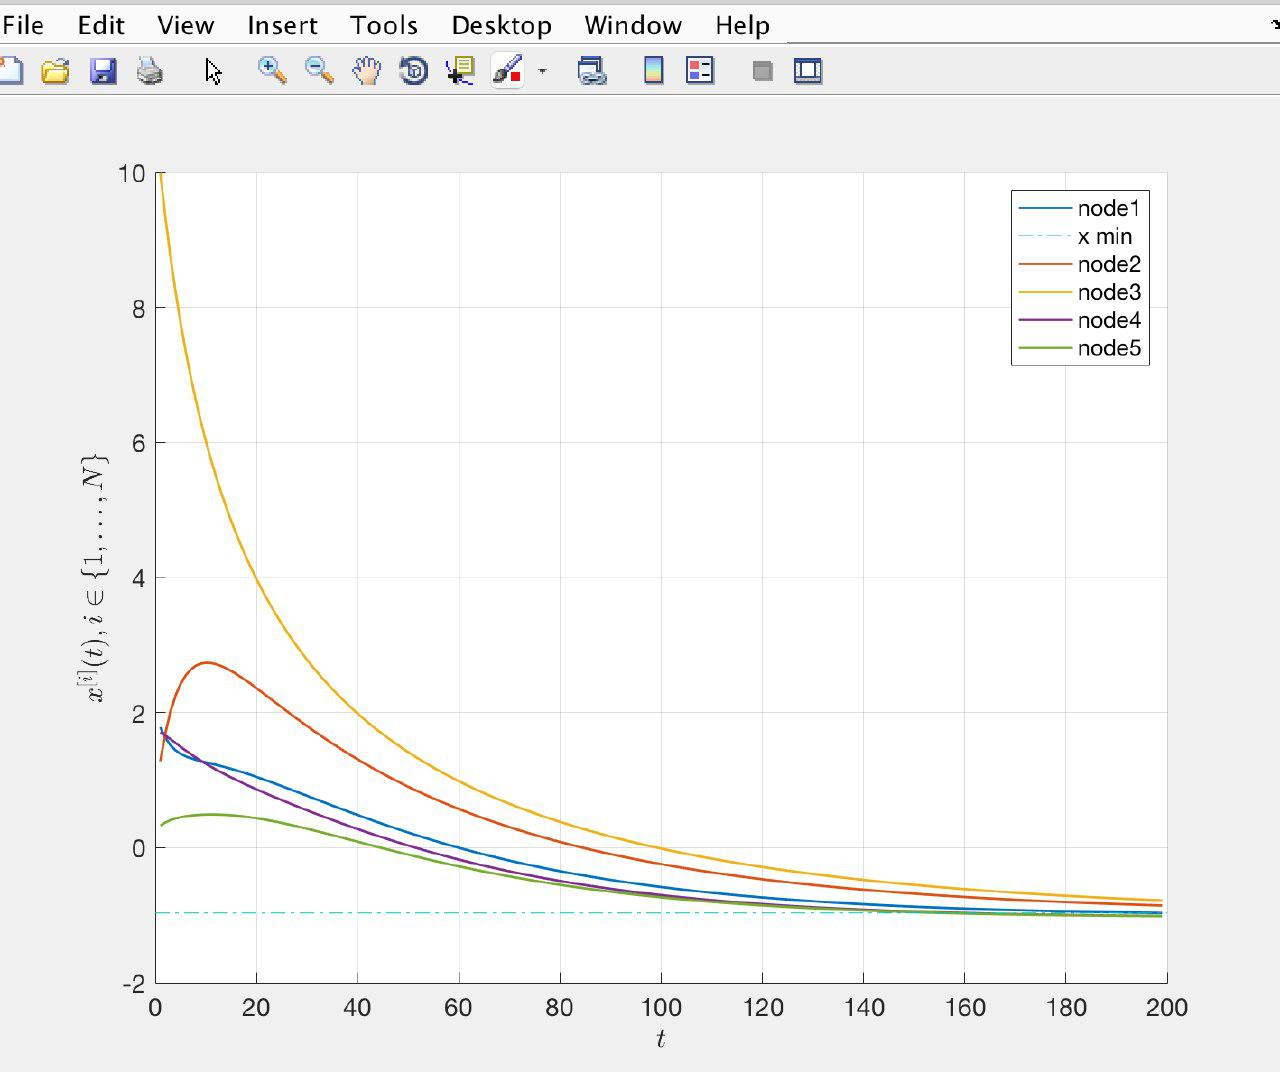
\includegraphics[width=8 cm]{caso1.jpg}
	\caption{$f_i(x)= x^2 + 1 +2x,\eta = 0.01, nodes = 5$ }
	
\end{figure}


\begin{figure}
	\centering
	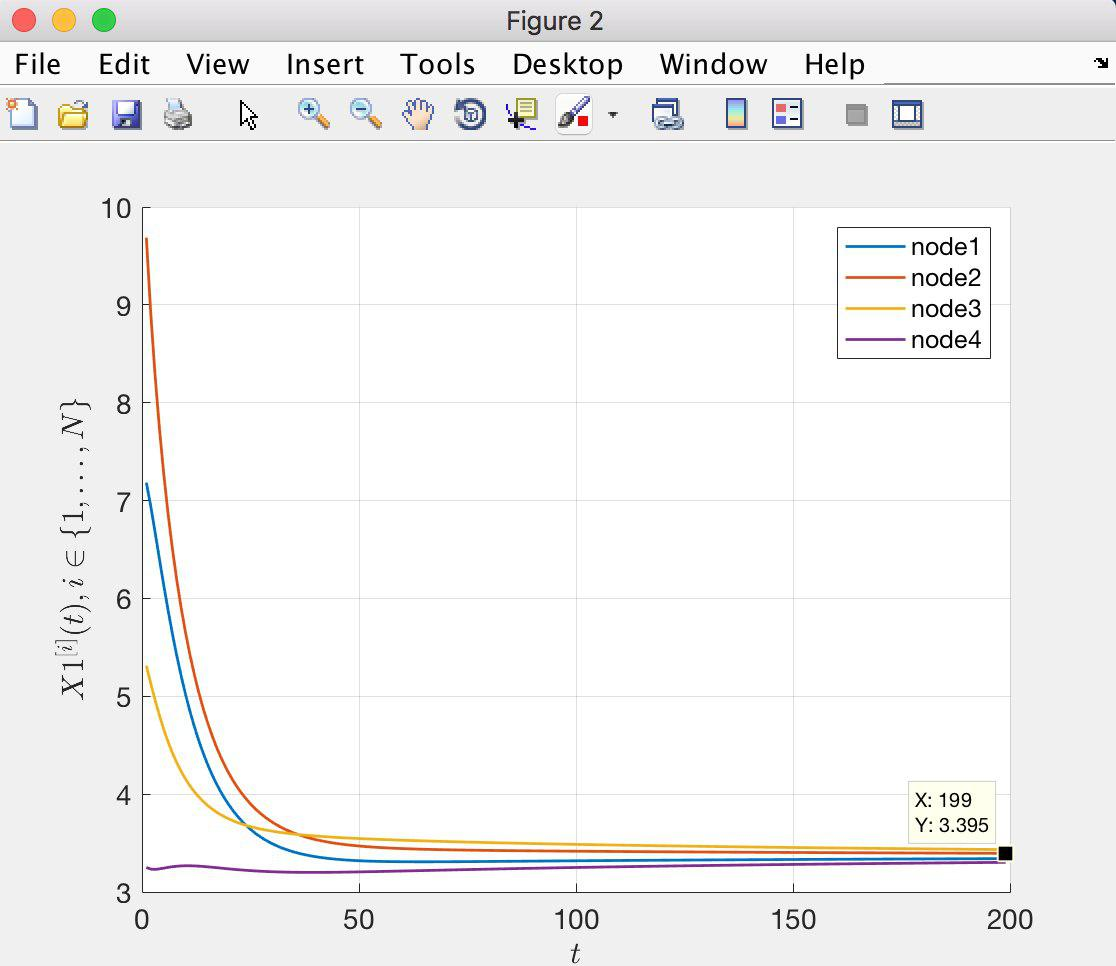
\includegraphics[width=8 cm]{caso2.jpg}
	\caption{X1, $f_i(x)= x_1^2 + 4x_2 + 1 - 2x_1 - 4x_2 +4x_1x_2 ,\eta = 0.01,nodes = 4$}
	
\end{figure}


\begin{figure}
	\centering
	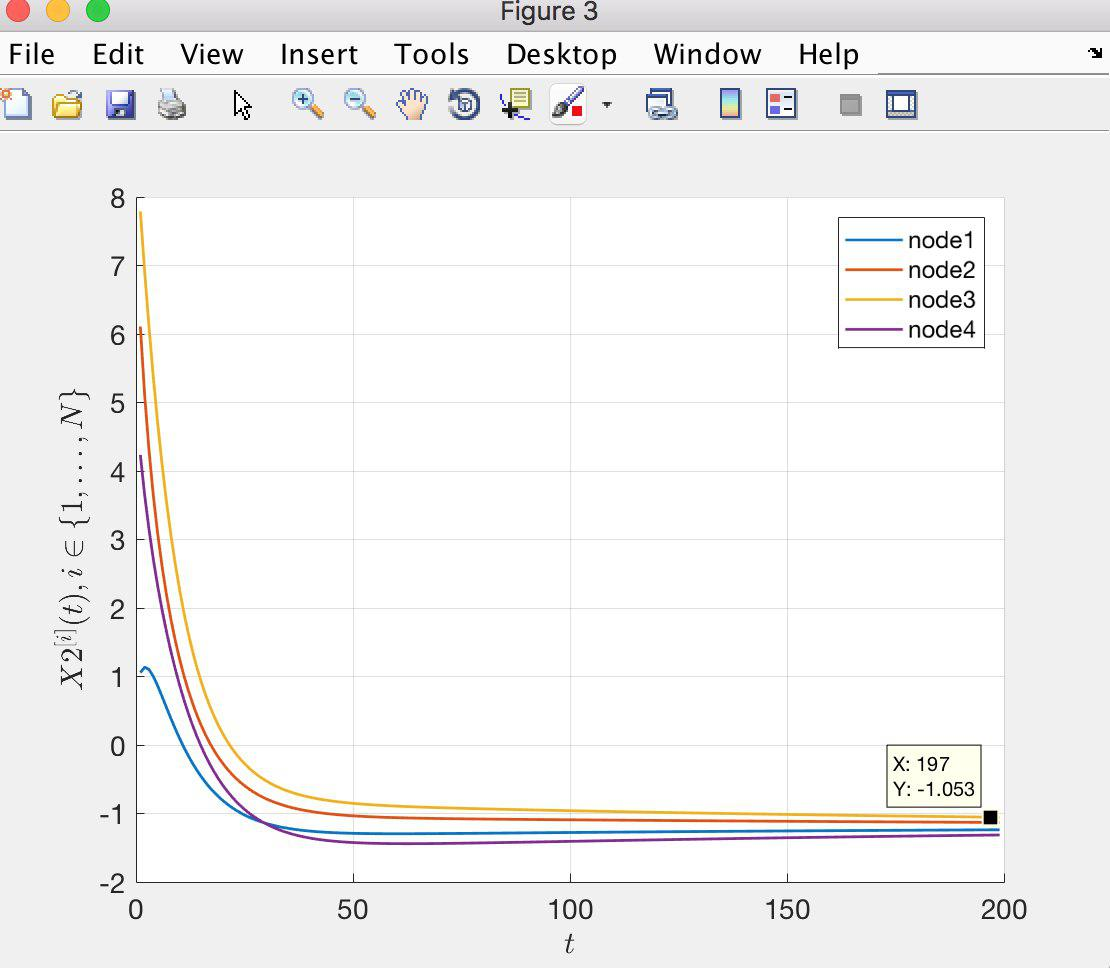
\includegraphics[width=8 cm]{caso21.jpg}
	\caption{X2, $f_i(x)= x_1^2 + 4x_2 + 1 - 2x_1 - 4x_2 +4x_1x_2 ,\eta = 0.01,nodes = 4$}
	
\end{figure}

\section{Pseudocode (Distributed Case)}
\small
{\linespread{0.33}\selectfont
\begin{itemize}
\item[]define number of agents, call it SIZE;
\item[]assign current agent to RANK;
\item[]If RANK = 0
\item[]~~~~check if user wants to solve a least square problem, call it ANS and 
\item[]~~~~broadcast it;
\item[]~~~~~~~~Case ANS = 'YES': get dataset points and distribute them to agents,
\item[]~~~~~~~~equally; 
\item[]~~~~~~~~Case ANS = 'NO' :
\item[]~~~~~~~~~~~get number of function components, $n$;
\item[]~~~~~~~~~~~get number of functions (1 or SIZE);
\item[]~~~~~~~~~~~get all functions;
\item[]~~~~define adjacency matrix, weight matrix and broadcast them to agents; 
\item[]For each RANK
\item[]~~~~get adiacency matrix $Adj$ and weight matrix $WW$;
\item[]~~~~define number of iterations (Maxiters);
\item[]~~~~get ANS and check for it;
\item[]~~~~~~~~Case ANS = 'YES' :
\item[]~~~~~~~~~~~get respective dataset portion;
\item[]~~~~~~~~~~~compute partial sum function wrt dataset portion, $f_i(x)$;
\item[]~~~~~~~~Case ANS = 'NO' :
\item[]~~~~~~~~~~~define n-size array of symbols;
\item[]~~~~~~~~~~~get the own n-dimensional function;
\item[]~~~~ initialize the state matrix $XX$ and the average gradient estimation $s$;
\item[]~~~~ assign random initial condition (at iteration 0), $XX(RANK,0)$;
\item[]~~~~ compute $ s(RANK,0) = \nabla f_i(XX(RANK,0))$;
\item[]~~~~ for $tt$ from 0 to Maxiters - 1 (for each iteration):
\item[]~~~~~~~~~set $U_{i1}$ and $U_{i2}$ = 0;
\item[]~~~~~~~~~destination = find neighbors of RANK, by reading $Adj$;
\item[]~~~~~~~~~for $jj $ = destination (for each neighbor of RANK):
\item[] ~~~~~~~~~~~~~~~$U_{i1}$ = $U_{i1}$ + $WW(RANK,jj)*XX(jj,tt)$; (for each component)
\item[] ~~~~~~~~~~~~~~~$U_{i2}$ = $U_{i2}$ + $WW(RANK,jj)*s(jj,tt)$; (for each component)
\item[] ~~~~~~~~~end
\item[] ~~~~~~~~~update the state of the agent, component for component:
\item[] ~~~~~~~~~XX(RANK,tt+1) = $U_{i1}$ - $\eta*s(RANK,tt)$;
\item[] ~~~~~~~~~update the average gradient estimation, component for component:
\item[] ~~~~~~~~~s(RANK,tt+1) = $U_{i2}$ + $\nabla f_i(XX(RANK,tt+1))-\nabla f_i(XX(RANK,tt))$; 
\item[] ~~~~end
\item[] end
\end{itemize}
\normalsize
\newpage
This pseudocode describes the software implemented using MPI for Python; in particular it starts with a node (rank 0) asking to the user if he wants to solve the least squares problem, or to find the minimum (if exists) of a given function.
\\ If the user choose the second option, it will ask if he wants to enter a single function, or to manually specify each $f_{i}$ (for each agent); if the user enter a single function then node (with rank) 0 will send it to each node. Note that the function/s are interpreted as symbolic arrays, so the user must respect Python syntax for mathematic operations in order to execute the software correctly.
\\ If the user wants to solve the least squares problem, then node 0 will read the dataset from a file, will divide the retrieved points in equal parts (if possible, otherwise  the node with highest rank will take the rest) and scatter them to each node. Node 0 will also broadcast the Adjacency and the weight matrices to all agents.
\\ Each node receives his set of points and then use it to compute the related function $f_{i}$ (remember that as written in Chapter 1, each $f_{i}$ acts as partial sum of the 'biggest' function to minimize).
From this point, regardless of the first user choice, the algorithm will proceed in the same way, with the agents that set the iterations, the stepsize, and initialize their initial state and their $s_{i}(0)$ values. At each iteration each agent communicates with neighbors, according  with the $Adj$ matrix, sending his state and the average gradient esimation at iteration $t$; with those informations, each node can now updates his state and gradient estimation before repeating the cycle until the end of the fixed iterations.
\\ Finally, each agent will have the same state (because they reached consensus); by substituting it in each $f_{i}$ we have the minimum value for each node: by summing all these values what we got is the minimum of the 'bigger' function obtained by summing all $f_{i}$ (in the case of the least square problem, is the function described in (1.5)).
\\ At the end the software plot the consensus achievement for each component of the state, the least square line (if the relative option in selected ).
\\The straight line $y = Ax + B$ in figure 2.4 was plotted using $X1$ and $X2$ respectively as angular coefficient ($A$) and the constant term ($B$). $X1$ and $X2$ are the components of the status vector with two rows and one column with the consensus values founds by our software.
\\The software plot on a file the difference (figure 2.5), for each iteration, between the function cost obtained from this software and the centralized version one (it use a Matlab library to compute the minimum of the same function).



\begin{figure}[H]
 \centering
 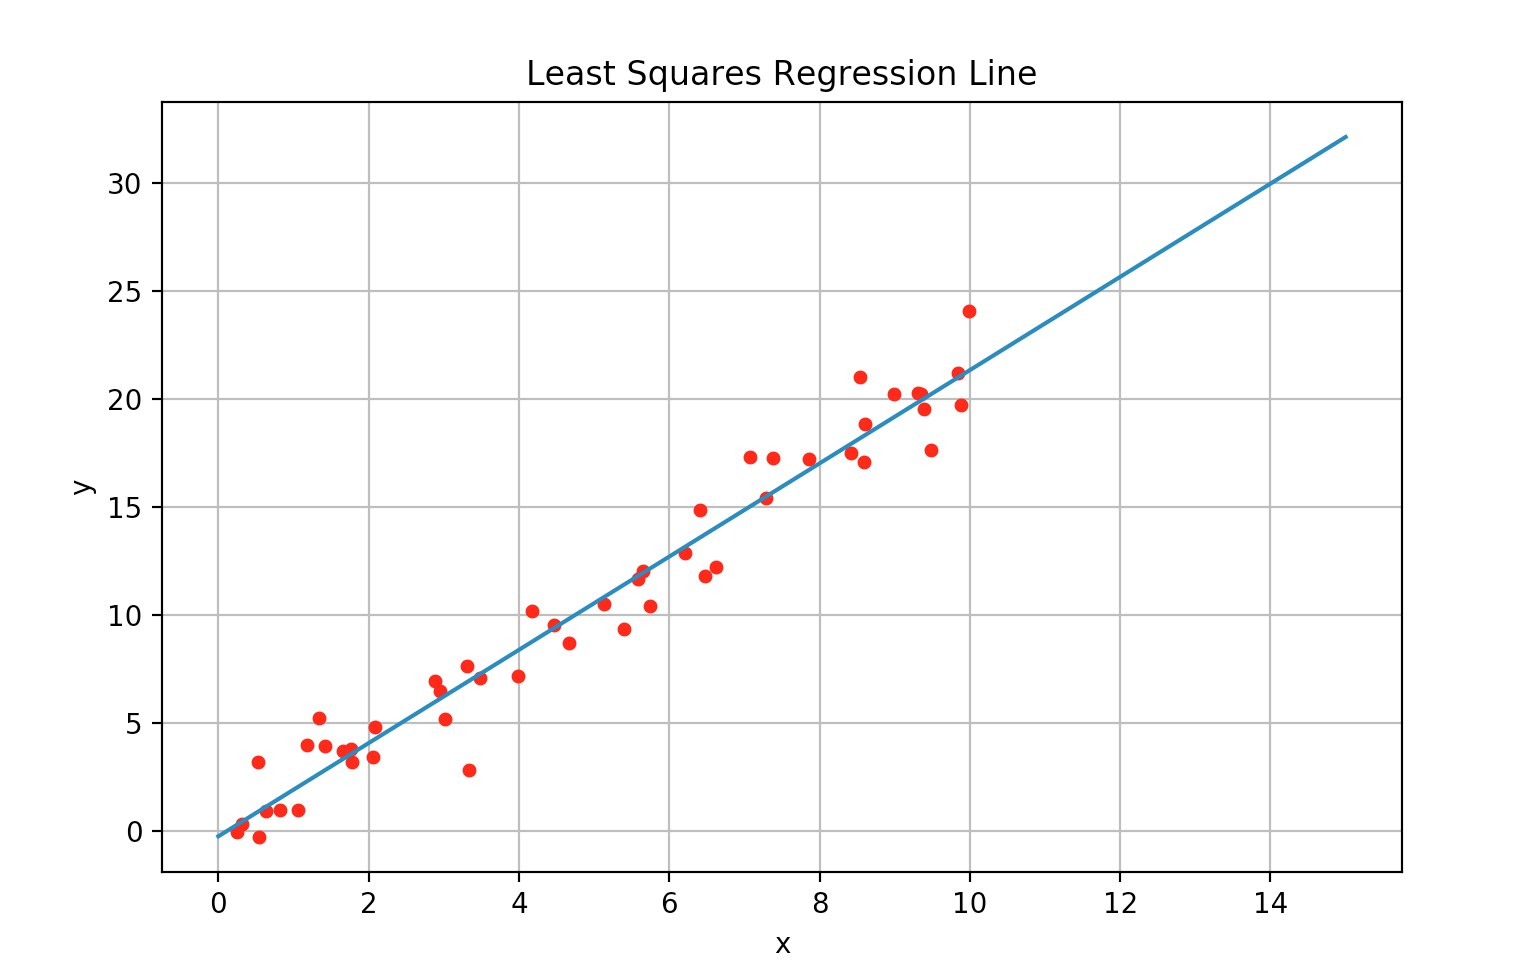
\includegraphics[width=14.5 cm]{figure5.jpg}
 \caption{$y = Ax + B, A = X1 , B = X2$, iterations = 1000, agents = 5}
 
\end{figure}

\begin{figure}[H]
 \centering
 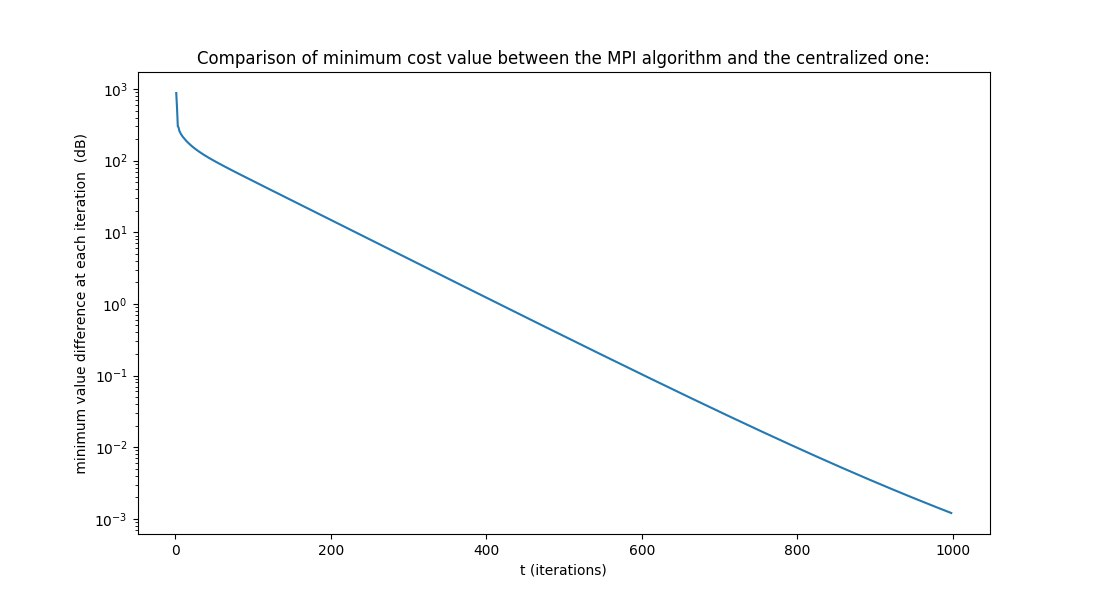
\includegraphics[width=14.5 cm]{figure6.jpg}
 \caption{difference between cost functions,  iterations = 1000, agents = 5}
 
\end{figure}



\section{Choice Of The Stepsize}
In order to assure the convergence of the algorithm the proper choose of $\eta$ is essential; taking $\eta$ too small will slow the convergence rate of the algorithm. To balance this effect, a solution can be to increase the number of iterations; in a distributed context this can be a problem because each single agent has to increase his iteration, and such a thing can decrease significantly the performance of the entire software.
\\ Instead, if we choose $\eta$ small, but not enough, the algorithm will diverge, and this is  even worse than the case described before. This is caused by the $\eta s_i(t)$ term in the update:
\begin{equation}
x_i(t+1) = \sum\limits_{j=1}^{n} w_{ij} x_j(t)-\eta s_i(t)
\end{equation} 
It acts as an average gradient estimation  times the stepsize, so if $\eta$ isn't small enough, the second term of (2.1)  becomes much bigger than the first; then the next update will be strongly influenced by the second term, and for $t$ big enough we will have something like this:
\begin{equation}
x_i(t+1) \approx -\eta s_i(t)
\end{equation} 
The first term will become  ever more smaller than the second one; each update $x_i(t+1)$ will be greater and greater in absolute value and even $\eta s_i(t)$ that depends both from $x_i(t+1)$ and $x_i(t)$. This behaviour cause a 'vicious cycle' in which  $x_i(t+1)>x_i(t)$ and $sign ~x_i(t+1)= - sign~ x_i(t)$; for $t$ big, $x_i(t+1)$ will goes to infinite.
\\ To avoid this situation a possibility is to choose $\eta$ that assure convergence for any number of agents ($n$): the minimum number of agents that we will considerate is two, so if $\eta$ is good for two agents, then will always be good; infact if we increase $n$, we will divide the function to minimize ($f$) into more parts ($f_{i}$), so each agent will have a smaller 'load', ( the coefficients of  each $f_{i}$ will be smaller) and this assure that $\eta s_i(t)$ (that also depends by each $f_{i}$ ) is small enough. However this choice of $\eta$ is the worst that assure convergence: suppose infact to take $\eta$ small enough for $n=2$ agents, increasing $n$, $\eta$ will remain fixed and the coefficients of each $f_{i}$ become smaller; so exists a $\eta_{x}>\eta$ for which $x_i(t+1)$, for $t$ big, will still converge. This $\eta_{x}$ will guarantee a better convergence rate then $\eta$ because $\eta_{x} s_i(t)$ will be greater than $\eta s_i(t)$, but small enough compared to $ \sum\limits_{j=1}^{n} w_{ij} x_j(t)$; so we will make a bigger step (respect $\eta$) along the average gradient direction, without going too far.
\\Our approach in order to choose a better fit $\eta_{x}$ was:
\begin{enumerate}
\item tried different $\eta$ values with $n=2$ for a given dataset;
\item we took the biggest $\eta$ that assure convergence;
\item adjusted $\eta$ testing it on several dataset (for $n=2$): in order to resolve the least square problem we found a good choice of $\eta$ by taking \\$\eta=0.0005$ and setting 600 iterations;
\item we tested different $\eta_{n}=\eta_{n-1}+\Delta\eta$ with $n>2$;
\item by attempts we found  a good choice by taking  $\Delta\eta$=0.0002.
\end{enumerate}
We computed each $\eta_{n}$ as :
\begin{itemize}
\item if (n$>$2)
\item $~~~~\eta=0.0005+0.0002*(n-2)$
\item else
\item~~~~$\eta=0.0005$
\end{itemize}
Notice that the relation between $\eta$ and $n$ is not linear,  our approach is based on attempts, so by increasing n over our computation capabilites (our test domain) it may happens that $\Delta\eta$ has to be adjusted to guarantee convergence.


\section{Weight Matrix}
Once generated the adjacency matrix and so the strongly connected communication graph $\mathcal{G}= (N,E)$, is required  a doubly stochastic weight matrix in order to reach the consensus between the $N$ agents (as described in the algorithm section); in our implementation of the distributed algorithm we tried two different weight matrix: the first one has been shown to us during an ACT exercise; the second (and definitive) is the lazy Metropolis, that is described in the assigned paper and that assure an high rate of convergence.
In particular the first one is computed as: 
\\$Laplacian = D - Adj$, where
\[
D = \begin{bmatrix} 
    deg(1) & 0 & \dots & 0\\
    0 & deg(2) & \ddots & \vdots \\

    \vdots & \ddots & \ddots & 0\\
    0 &  \dots & 0 &  deg(N)
    \end{bmatrix}
\]
$D \in \mathbb{R}^{{N}\times{N}}$, got the degree of each agent $deg(i)$, namely the number of his out-neighbors, (note that in our case $Adj$ is symmetric because we want an undirected graph, so the out-degree is equal to the in-degree); $Adj \in \mathbb{R}^{{N}\times{N}}$. Then the weight matrix $WW$ is given by: 
\begin{equation}
 WW= I - 0.05*Laplacian
\end{equation}
with $I\in \mathbb{R}^{{N}\times{N}}$. In general, for this $WW$, the elements on the diagonal assume a much higher weight than the respective neighbors; this can influence the convergence rate of the algorithm because more iterations are required to reach consensus.
\\ To get a better convergence rate we decided to substitute the $WW$ described above, with the matrix proposed by Guannan Qu, Na Li on their work: the lazy Metropolis. In this matrix each $ww_{ij}$ is computed as:
\begin{equation}
 ww_{ij} =
   \begin{cases}
   \dfrac{1}{2~max(deg(i) , deg(j))}~~~~~~~~if~ i\neq j,~ (i, j)~ connected.\\\\ 1 -\sum\limits_{q \in N_{i}}\dfrac{1}{2~max(deg(i), deg(j))}~~~~~~~~if~ i = j.\\\\0~~~~~~~~~~~~~~~~~~~~~~~~~~~~~~~~~~~~~~~~~~ elsewhere.
   \end{cases}
\end{equation}
Where $N_{i}$ denotes the set of neighbors of agent i ($card(N_{i})=deg(i)$).
Below is shown the agents consensus achievement in function of $t$ for both $WW$  :

\begin{figure}[H]
 \centering
 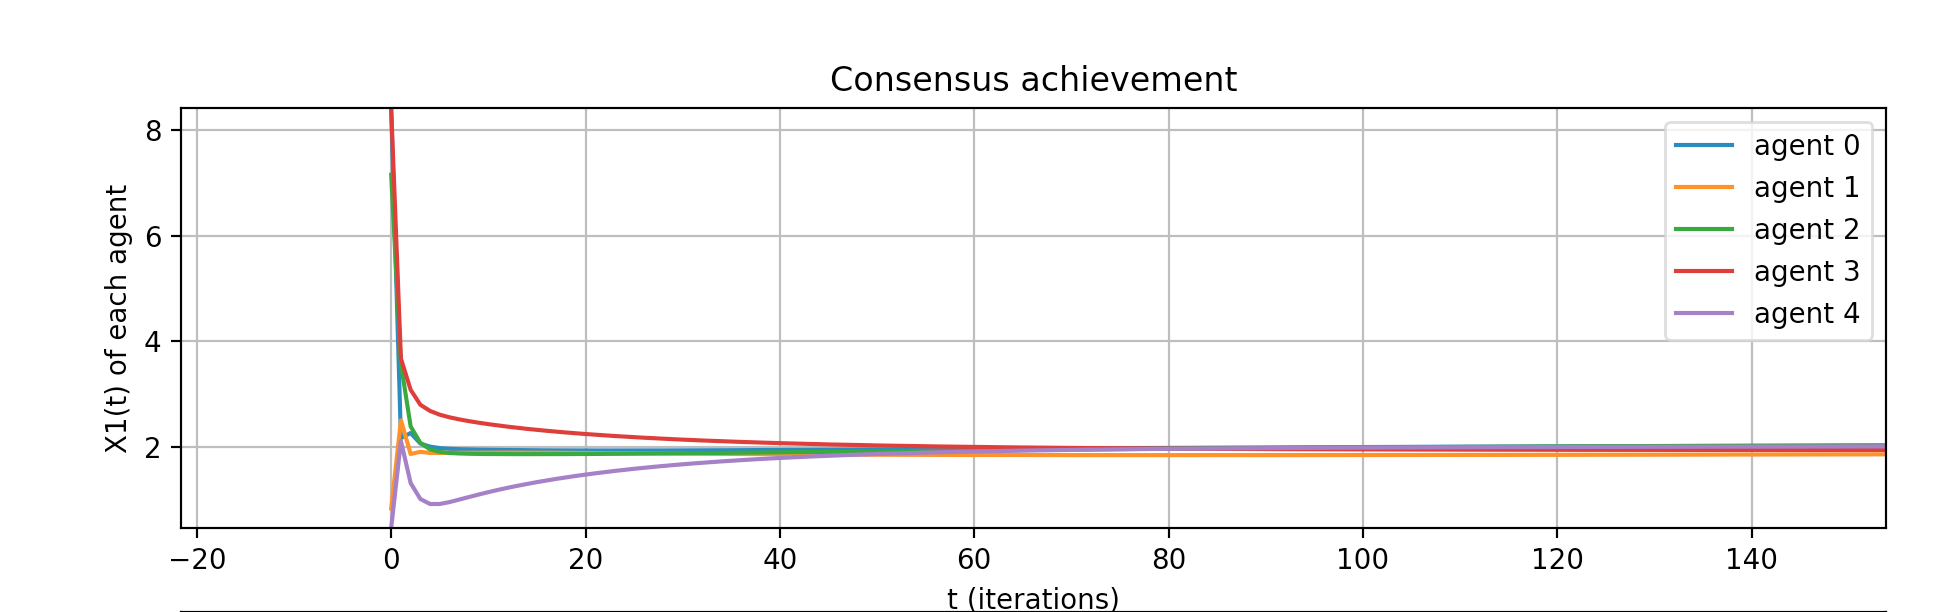
\includegraphics[width=14.5 cm]{ww.jpg}
 \caption{consensus using the first $WW$, iterations = 600, agents = 5}
 
\end{figure}

\begin{figure}[H]
 \centering
 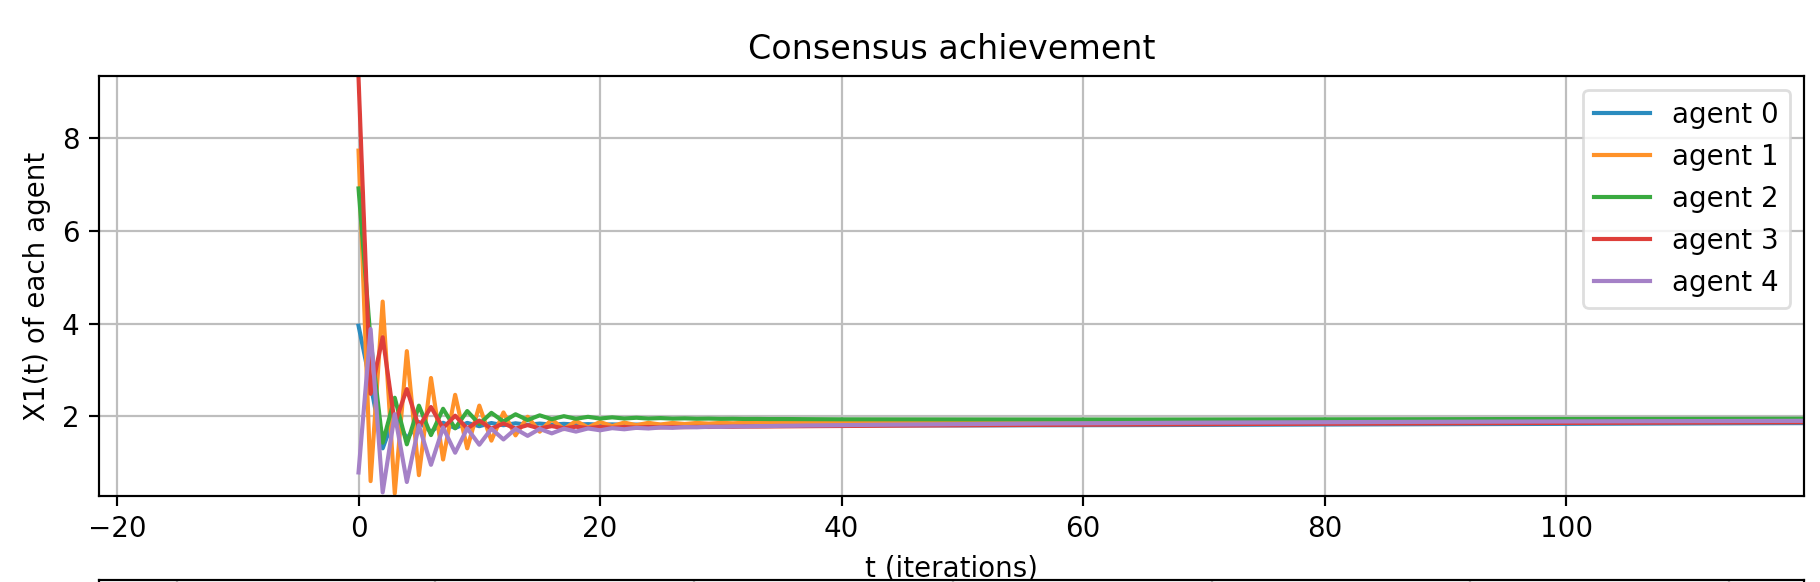
\includegraphics[width=14.5 cm]{lazy.jpg}
 \caption{consensus with Metropolis $WW$, iterations = 600, agents = 5}
 
\end{figure}

\section{Scripts}
Our project consists of different scripts that we wrote in a  modular structure: \\\\$"dataset\_generator.m"$ is a Matlab function that calls:\\$"Linear\_regression\_dataset.mat"$ (given in the Group 5 folder) and use the $"Readme.txt"$ content to generate the points of the dataset.  When user invokes $"dataset\_generator"$ new points are generated and saved on a file.\\\\
 $ "min\_central"$ is a Matlab function based on the "fminsearch()" tool : it find the minimum value of a given  symbolic function; the result will allows to compare the minimum value of the MPI software with the Matlab built-in solver one , (see graph in figure 2.5). \\User can call $ "min\_central(function,number of components)"$ specifying the symbolic function, (to make a reasonable comparison, it has to be the same function that MPI software has to minimize) or an empty string ("") in the case he wants to solve the least squares problem. In this last case $ "min\_central"$ read the dataset written by $"dataset\_generator.m"$, compute the partial functions, and then it sum them, obtaining the 'bigger' function to minimize. In both cases, print the minimum value on a file.
 \\\\$"mpi\_min"$, a Python script, is the central part of the project. It is the MPI software described by pseudocode; it reads from a file the $ "min\_central"$ minimum value and the dataset created by $"dataset\_generator.m"$ by using the script $"ret\_data"$; then: 
 \begin{itemize}
 \item compute $Adj$ matrix using the  $"system\_ADJ"$ script;
 \item compute the weight matrix using $"degree\_MTX"$ (by passing two different parameters you can use Lazy metropolis or the original weight matrix);
 \item calls $"partial\_sum"$ to assign to agents their own partial sum.
 
 \end{itemize}
 
 
$"solver\_min"$ is the non-distributed version of  $"mpi\_min"$, it simulate the agents communication using a for-cycle. We used it as grounds for $"mpi\_min"$.
\\\\$"exec\_proj"$, a  Matlab script that minimize a function $f(x): \mathbb{R} \rightarrow \mathbb{R} $, it represents the starting point of the project.

%%%%%%%%%%CONCLUSIONS%%%%%%%%%%
\chapter*{Conclusions} % and future developments}
\addcontentsline{toc}{chapter}{Conclusions} %  and future developments}
This work has arisen the design and the implementation of a software system for solving distributed optimization problems. The algorithm used has been developed in [1], based on the average gradient estimation.\\
After a fully understanding of the mathematical concepts from first chapter, chapter two focus on the implementation aspect; in order to satisfy complete requirements list, complex problem has been split into more simply task and the results are consistent with the theoretical results.\\
From the point of view of the implementation, the choice to use Matlab for preliminary steps and Python as programming language for our software is due to the python characteristic of a non-type language and so, it is more oriented to manage particular implementative requirementes.\\
About distributed management, the library used has been Mpi4py by which have been used the most common functions for messages exchange among agents.\\
The obtained results are good and possible future developments arise to ensure a greater accuracy and a higher hardware efficiency.\\\\\\
This project helped us to better understand the optimization problems class and the way to distribute them. In particular we deepen some aspects related to agents communication, and in the way this can lead to a consensus among them.

%%%%%%%%%%BIBLIOGRAPHY%%%%%%%%%%%
\bibliography{Bibliography}{}
\bibliographystyle{plain}
\addcontentsline{toc}{chapter}{Bibliography}
%%%%%%%%%%%%%%%%%%%%%%%%%%%%%%%%%%%%%%

\end{document}
